
\documentclass[english]{tktltiki}
\usepackage[pdftex]{graphicx}
\usepackage{graphicx}
\usepackage{subfigure}
\usepackage{url}
\usepackage{xcolor}
\usepackage{amsmath}
\begin{document}


\onehalfspacing
\title{Reinforcement Learning in Games: A Mini Survey}
\author{Ege Can �zer}
\date{\today}

\maketitle
\numberofpagesinformation{\numberofpages\ pages + \numberofappendixpages\ appendices}

\classification{\protect{\ \\
	A.1 [Introductory and Survey],\\
	I.7.m [Document and text processing]}}

\keywords{Reinforcement Learning}

\begin{abstract}
    Self-learning programs have been studied and applied in many different fields; but recently, it gains more popularity and familiarity due to its breakthrough success in the game domain. Unlike the examples are taken from the real world, having the predefined set of rules and the less complicated environment in this domain provides greater flexibility to develop reinforcement learning algorithms. In this paper, we will study the applications of reinforcement learning algorithms in the game context by closely focusing on four different articles. Based on the findings, we hope to propose possible improvements for future studies.
\end{abstract}

\mytableofcontents

\section{Introduction}
During the last decade, Reinforcement Learning (RL) paradigm, despite being actually not a new concept, has gained decent amount of popularity. Starting from middle 80's and ever since then, it has been applied in many fields to address complex problems such as in robotics, control systems, finance, and agent-based systems due to its generic formulation. In its essence, RL concept looks for optimal input actions that maximizes the output states by making use of the feedbacks from environment \cite{tesauro1995temporal}. In spite of the fact that RL being a mature and widely-used concept, the primary reason to get such attention recently is due to breakthrough success in the game context \cite{mnih2013playing, silver2016mastering}.

Studying RL algorithms in the game context contributes several definitive advantages \cite{tesauro1995temporal}. In general, modeling of the problem, implementation, and analysis of the results in real life examples are harder than the artificial ones such as games. Moreover, having simplified and controlled environment, as well as specifically defined rule sets not only allow an opportunity to explore the new variety of RL algorithms, but also enable to have concrete evaluation measurements. Further, research results are reproducible, easy to simulate and provide test-bed for future studies. Therefore, for the given reasons, studying RL in games can help the field to progress further and more effectively.

Advancement in a scientific field affect one to another and grants to improve even more towards advancement; the notion enables opportunity to observe the advancements, yet to come, obtained by the RL in games. The usual case is where the previous developments leads to a new one, such an example appears in the article by Gerald Tesauro \cite{tesauro1995temporal} that combines neural network and temporal difference concepts into new one. Another case is that advancements in the related fields drive a new one. For example, Mnih et al. \cite{mnih2013playing} proposes a deep learning model that learns control policies directly from sensory(image, video) input, which made it possible by computer vision and speech recognition research fields. As a matter of fact, this mini survey, in some sense, will explore the final case that how RL in game context can affect the other fields. That is, playing patterns of such artificial intelligence can provide knowledge on how to progress towards advancement.

In this paper, we will review four different existing reinforcement learning systems in the game context. The rest of this paper is organized as follows. In section 2, we discuss common challenges and approaches to the problems in RL in games such as dealing with abstraction of the environment or evaluation of the results. In section 3, we review existing systems in detail each with its unique characteristics. Then following section proposes possible improvements that can be taken to improve the research field. Last section summarizes and concludes the paper.

\section{Challenges and  approaches}
In the last decade, many research has gone into investigating reinforcement learning algorithms in the game context. Concurrently, many challenges and approaches have arisen around this topic repeatedly. In this section, we present some of those common challenges and some approaches that exist mostly in the reviewed systems \cite{tesauro1995temporal, amato2010high, liao2012cs229, mnih2013playing}.

Because there exist many different and specific problems as well as methods to tackle them, the challenges and approaches listed in this section are all related but not necessarily belong to every system in the whole research field. Generally, given matters are all common, but still some of them may not appear within another context.

\subsection{Implementation point of view}
The fundamental necessity to find a proper playground to study reinforcement learning algorithms in the game context certainly unignorable. Nonetheless finding the platform, implementing it through the given medium, and evaluating the results may differ. Moreover, it limits the researches due to the lack of freedom in the provided software. So it may ending up building the whole playground from scratch, which surely is a wrong way to start to study the algorithm. Therefore, finding appropriate software development kits (SDKs) are crucial even before considering the study the RL algorithms in this domain.

Fortunately, there exists plenty of variety in the approach to implementation, ranging from turn-based board games to fast-paced action games. It is reasonable to not expect to have every games mainly due to the trademarking concerns; but still some open source the contents or provide refined framework for everyone. For example, we observe \cite{amato2010high, liao2012cs229, mnih2013playing} take advantage of several SDKs/frameworks that they use to apply the algorithm to train the agent and even to evaluate the results. In addition, we recently recognize different and more self-aware general AI training way per se. However, we will discuss the matter in the section 4. In all, having a proper medium to study these algorithms is not negligible and certainly important aspect in this context.

\subsection{Abstracting the environment}
In order to study the games properly using reinforcement learning, certainly the very first step is abstracting the game environment in terms of Markov decision processes (MDPs). Since the modeling choices, as well as the definitions may differ based on the systems (for example, transition probability parameter does not exist in Q-learning). Therefore, we will follow an example model by Liao et al. \cite{liao2012cs229} to only illustrate the concept. Besides, we are not going to give in-depth algorithmic analysis for any of the inspected systems in this paper.

\begin{align}
Q(s_t, a_t) \leftarrow 
(1 - a_{s,a}) Q(s_t, a_t) + 
a_{s,a}(r + \gamma max(Q(s_{t+1}, a_{t+1}))) \label{eq:mario}
\end{align}

We can inspect the required elements for a model more easily directly from the equation \ref{eq:mario}. In total \textit{five} factors need to be defined in this model. Those are $ s_t $ state space that the agent might be in, $ a_t $ set of actions that agent capable of, $ r $ reward function that the agent receives after transitioning from $s_t$ to $s_{t+1}$ via $ a_t $. Then, $\gamma \in [0,1]$ discount factor serves as tuning parameter for present and future rewards, and finally $ a_{s,a} \in [0,1]$ is learning rate that affects agent's converging rate, further details are stated in \cite{liao2012cs229}.

By using the provided AI application interface, Liao et al. \cite{liao2012cs229} encodes the game environment--Mario in the following way. From the figure \ref{fig:mario} it can be inferred that nearly any condition of the character and its surroundings can be extracted. According to the article, $s_t$ designed in a way that it requires 39 bits to encode in a state vector, such example attributes are Mario's current mode (small, big, fire), movement states, enemy distance within 3 different ranges and so on. There are 12 different $a_t$ that Mario agent can perform, from the combinations of (LEFT, RIGHT, STAY) x (JUMPY, NOT\_JUMP) x (SPEED/FIRE, NO\_SPEED). In the article $r$ is defined as combination of weighted state attribute values and the distance that agent performs from the last frame. $a_{s,a}$ and $\gamma$ parameters chosen based on several try-outs that would lead to non-degenerated performance in the evaluation.

Over-all, we revealed an example approach to encode a game environment to be able make use of a reinforcement learning algorithm. Moreover, there are many ways to handle the abstraction of game environment and making use of the RL algorithms, which we will cover these later on. However, we briefly categorize them in 3 possible ways, low-level, high-level and context-free abstraction/modeling based on the systems we reviewed. We refer the presented approach as low-level abstraction where the designer have access to nearly all attributes available. If one can access only the limited resources and be able to utilize inner mechanics of the system we refer this as high-level modeling. Context-free modeling encodes the environment without any context related knowledge. In the literature we observed that such modeling can achieved by using convolutional neural networks \cite{mnih2013playing, silver2016mastering}. We will go over those as we review systems in the further sections.

\begin{figure}[h]
	\begin{center}
		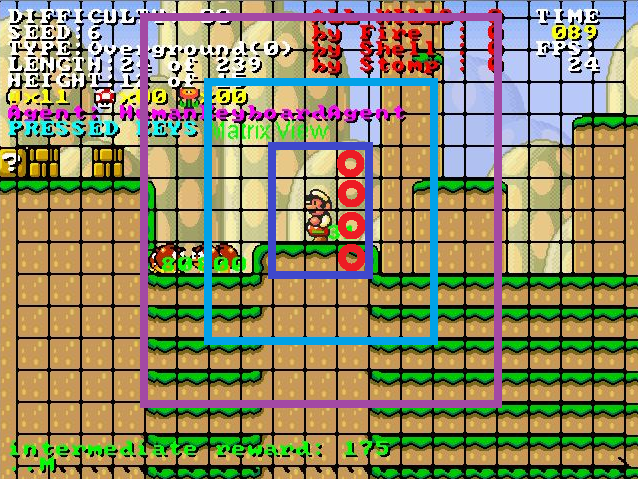
\includegraphics[width=0.65\textwidth]{img/mario.png}
		\caption{ Mario's scene \cite{liao2012cs229} }
		\label{fig:mario}
	\end{center}
\end{figure}



\subsection{Performance measures}
In the many of the sub-branches of the machine learning area there is one thing in common; how actually good our model is. By the nature of "learning by experience" in the reinforcement learning, it is hard to provide many hand-crafted ground truth, compared to supervised learning. Because it takes thousands and even millions of iterations to have an intermediate to expert level of agent. Thus, one needs to consider other means of evaluation.

There are several different methods available to assess the quality of the model; however, we consider the groups that Gerald Tesauro \cite{tesauro1995temporal} states. According to this, we mention there are three different methods to evaluate RL model. It is high-level, general enough to cover most of the systems, and actually used without a naming convention by others. Also for this paper, we will refer these groups in our comparative analysis later on.

First method is evaluating the system using automated benchmarking system. This can be seen as a computer opponent, or an objective platform for all other AIs. One obvious advantage of using these kind of automated tool is that the programs can be iterated over many times and accurate statistics can be obtained to support sufficient benchmarks.

Second method is evaluating the system against the master level human players. The major benefit of this method is that it can serve as clue about the reference point of a play performed by the system. However, as the level of complexity increases in the games, the human knowledge may be erroneous and thus unreliable to serve as a ground truth. This seems to be happen frequently in the history especially in the board games such as \cite{tesauro1995temporal, silver2016mastering}. Also, the number of game plays against humans are more restricted and slower, specifically compared to previous one. But, the evaluation method still can aid for the given reason.

Last evaluation method is done by analyzing individual decisions by system, which is actually closely related to the second method. Moreover, it is valid to say that it also inherits nearly the same problems. Gerald Tesauro \cite{tesauro1995temporal} states that the method used to analyze the individual decisions via computer roll-outs in a backgammon game. However, one can induce this approach for any systems. The key thing is to set up candidate positions, just as in the supervised learning, and letting the computer to play out the position several times. The results can be deductible from the statistics of good and bad plays. However, it is more suitable for stochastic environments or having large state spaces, generally board games. 

\subsection{Further challenges}
Until now we bring up usual common problems that every reinforcement learning systems strives. Still, underlying all possible challenges, especially after the combinations of other fields, not only out of scope of this paper but also is intractable and demanding task. For this reason, we will additionally cover only a few prominent ones from what we have studied. Briefly these are: exploration versus exploitation trade-off and various RL challenges from deep learning (DL) point of view.

To begin with, exploitation versus exploration dilemma is truly one of the classic challenges in the reinforcement learning. Problem comes along with the agent's main learning objective. That is, the agent must be able to obtain the maximum possible reward from the actions that it has performed before. Still, it must discover such new actions that would also lead to maximize the reward in future \cite{sutton1998introduction}. The dilemma is basically deciding on what is the perfect moment to explore and exploit, yet it has no single solution. Sutton and Barto \cite{sutton1998introduction} demonstrate ways to balance between exploration and exploitation, including $\varepsilon$\textit{-greedy} and \textit{softmax} which all are perform near-optimally reward. Even though there exists many possible techniques in the literature, upon closer examination $\varepsilon$\textit{-greedy} appears to be common approach, also in \cite{amato2010high, liao2012cs229}.


On the other hand, RL suffers many problems from DL point of view which some are identified by Mnih et al. \cite{mnih2013playing}. First, data needs to be independent and identically distributed based on the assumptions of DL algorithms. In contrast to this, RL usually consists of sequences of highly correlated actions. Moreover, vast majority of DL algorithms requires extensive amount of labeled data to achieve "automatic" feature extraction, whereas RL algorithms' experience-based learning demands reward that is usually noisy and delayed. Also, agents in RL algorithms likely to change their behaviors as they explore, this indefinite data distribution violates the fixed distribution assumption of the DL algorithms. Fortunately, there exists deep learning approach to overcome these issues \cite{mnih2013playing}.

\section{Review of existing systems}

Until now we have seen that there are several challenges and approaches for the reinforcement learning algorithms in the game context. In order to give more insight about the challenges and approaches, we have examined four unique systems in this section. We hope to demonstrate their adaptation to the challenges, how do they handle and make use of the reinforcement learning in this domain. At the end, table \ref{table:comparison} summarizes the properties of articles.

\textbf{\textit{Reinforcement Learning to Play Mario \cite{liao2012cs229}}}

First article authored by Liao et al. \cite{liao2012cs229} focus on the design of single agent to play classic platformer game called Super Mario Bros using $\varepsilon$\textit{-greedy} Q-learning. The aim of the agent is to get the highest score and also to overcome various obstacles and rewards such as beating enemies, avoiding gaps, or collecting items until it reaches to finish line.

Mario AI framework interface aids to abstract the game environment at low-level, meaning many attributes tailored to encode into one state. Main motivation to use the $\varepsilon$\textit{-greedy} Q-learning algorithm, instead of "normal" RL, is because the state transition probabilities do not need to be known by the algorithm beforehand. Moreover, the method ensures larger state space and faster computation time. $\varepsilon$\textit{-greedy} action selection extension provides balanced way to explore more states, as well as decaying learning rate ensures faster converge policy rate than fixed learning rate. 

Using the same framework, training and evaluation of the agent are done under different learning parameters. The optimum one is selected based on the four performance metrics. After 5000 training iterations the agent is able to reach approximately 90\% of winning probability ($\approx$ 9000 average score) of the game. On the other, evaluation of the system is only compared against baseline. Even though the tool by Karakovskiy and Togelius \cite{karakovskiy2012mario} provide several benchmarking tracks, none of the performance metrics present an objective comparison to existing systems. To be able to present definitive results, a possible benchmark or a human-level comparison could be applied. 

\textbf{\textit{High-level Reinforcement Learning in Strategy Games \cite{amato2010high}}}

Second article, Amato and Shani \cite{amato2010high} study to improve the built-in AI of a turn based strategy game called Civilization IV using high-level RL learners. The single/multiple can accomplish this by switching between high-level strategies of "leader traits", and leaving the low-level actions (technology investment, unit creation etc.) to the built-in AI. To begin with the abstraction of the game environment, states are defined in terms of the resource values, namely population difference, military power, land difference, and remaining land. Then, action space is based on the four leaders that have all possible variety of leader traits, such as financial, aggressive and so on. Lastly, reward model is based on the built-in scoring heuristic of the game, by which score difference of players used as the reward. 

Article compares three RL algorithms, particularly Q-learning, Dyna-Q, and Dyna-Q with conditionally independence assumptions between states. Evaluation of the algorithms done by comparing with the build-in AI under distinct leader match-ups. After different training episodes, overall Q-learning performs worst, the former Dyna-Q best, the latter one second due to obvious state dependency between transitions, but still performs better than Q-learning and faster than the usual Dyna-Q. Nevertheless, they all perform better than the built-in AI, which means RL even can contribute to environments such that it is highly complex and the low-level behavior cannot be adjusted. 

One side note, considering each leader has different initial advantages, match-ups could also be organized in a way that the designed agent has the less favorable one, a mirror match-up with increasing difficulties of built-in AI (Prince to Immortal level), or to test the multi-agent capability a team match-up could be planned. With the current evaluation scheme (limited leaders and match-ups) only finite number of approaches to win a game can be observed.

\textbf{\textit{Temporal Difference Learning: TD-Gammon \cite{tesauro1995temporal}}}

So far we discussed two systems that have converged into decent results either by exploiting the heuristics and/or with the aid of built-in AI. Gerald Tesauro \cite{tesauro1995temporal} presents a temporal difference (TD) neural network learner that trains itself and automatically discovers the features where agent able to reach world-class human grandmaster level in the backgammon game.

Initially, the total number of checkers, from only one side, are vectorized according to each position on the board. This representation is then given as input pattern to NN, which also has output patterns consisting of 4 possible outcomes for example a white win by gammon. At each time step, edge weights of NN is calculated by using TD($\lambda$) algorithm. By the end of game, again  the "outcomes" given as the final reward for weight calculation. 

In the training phase, agent makes the move for both sides and scores possible legal moves, without any heuristics, at each step in NN. Then from NN maximum likely outcome is selected to make the next move. This learning methodology with no heuristics managed to reach at intermediate-level of play. Yet, after adding hand-crafted features and training for about 1.5 millions of self-played game, TD-Gammon achieved master level of play \cite{tesauro1995temporal}.
\\

\textbf{\textit{Playing Atari with Deep Reinforcement Learning \cite{mnih2013playing}}}

Heretofore, game specific information would needed to be encoded such that diverse RL algorithms could make progress towards learning. Mnih et al. \cite{mnih2013playing} introduce a context-free method called \textit{deep Q-network (DQN)}, that is a combination of CNN and RL by which the model takes information nothing but from the video input. Their approach overcome several challenges between RL and DL, as we discussed in the previous section.

First of all sensory inputs taken from Atari games consist of high dimensional frames, therefore, preprocessing is crucial to reduce observation dimensionality. Then, a state is described as the sequence of observation and action pairs, because it is impossible to completely relate the situation from only one observation. However, this scheme can cause the training sample to dominate others, especially if the maximizing action is only particular one. For example, if the maximizing action that moves to right, then it dominates the other actions. For that reason, experience replay mechanism is used to smooth out the sample distributions. Moreover, Q-learning is used for the same rationale, meaning unlike the on-policy learning like SARSA, off-policy updates Q-values using the greedy action not current policy's action. Actions are executed based on $\varepsilon$-greedy policy, after that the reward and next frame is observed then stored in the replay memory. In order to alleviate the relating independence assumption in DL; that is, correlations of consecutive samples are randomized at each step in the replay memory. Finally, gradient descent is performed to calculate the local minimum of the network.

The system played 7 Atari games using Arcade Learning Environment. According to results, DQN outperforms all RL algorithms, whereas at only 3 games the system exceeds human performance for the remaining games, the result is far from being close.

\begin{table}[h]
	\begin{center}
		\hspace*{-1.25cm}
		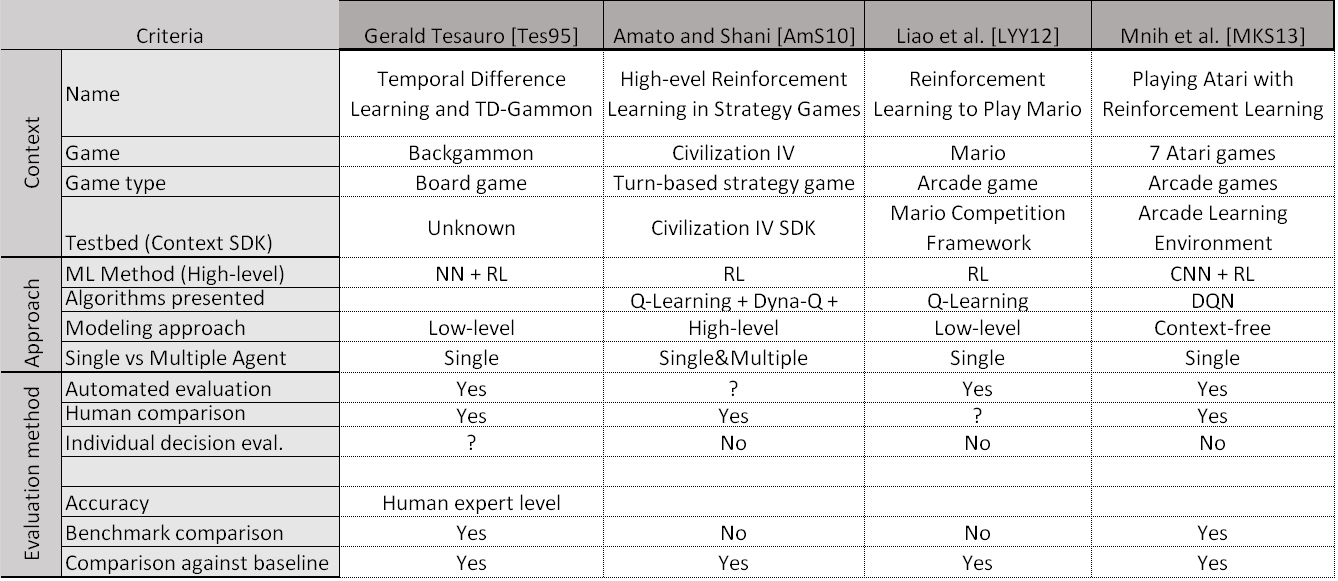
\includegraphics[width=1.1\textwidth]{img/comparison.png}
		\caption{DRAFT! Comparisons of the systems }
		\label{table:comparison}
	\end{center}
\end{table}

Explain the table and express your findings about the reviews. For example context specific outcome

 But surprisingly, upon further analysis by Pollack and Blair \cite{pollack1997did} it is concluded that the main reason to achieve this level of play was not related with the TD and NN approach, but the self-playing scheme and the stochastic environment of the backgammon game. This finding led us to question the other systems that may have context specific performance regardless of the algorithm, which we will discuss later on.
\newpage
%\section{Future research}
%
%\colorbox{red}{VERY FIRST DRAFT}
%
%\begin{itemize}
%    \item Sandbox learning, can this be used to train DQN approach and applied on other games? This way one may not to deal with the context at all? RL in games, may help other. Studying real-time/complex video games is hard due to lack SDK. Mainly, algorithms implemented on these game because they were the only available one. The need for the general AI trainer play ground Sukhbaatar et al. \cite{sukhbaatar2015mazebase}. Find the example that makes use of this (cannot find the paper atm. Starcraft AI player trained outside of the context i.e. by this sandbox).
%    \item Getting around with the context specific information, if we can overcome this, it is likely to have \textbf{general purpose learner} that can be trained such that can achieve anything, because NN can achieve fixed accuracy under X iteration?
%\end{itemize}
%
%\subsection{Context specific outcomes(include this in future)}
%\colorbox{red}{HIGHLY INCOMPLETE DRAFT}
%
%Mastering the game of Go with deep neural networks and tree search \colorbox{red}{Find papers}
%
%Even though a new algorithmic concept provides certain solution, for a certain context it may not necessarily give comprehensive solution for every other systems and possibly may lead to wrong direction.
%
%Found some articles discusses the solution of TD-Gammon did not work out well for other games. Results of
%some games in \cite{mnih2013playing} also proves that. Which brings the question AlphaGo is surely a success, but does that mean it is success for not something big? Only for that particular solution? We will see that.
%
%"Playing atari paper" points out the TD-Gammon problem due to its stochastic dice rolls, using the same argument, it can also be inferred that AlphaGo's technique is also target specific, i.e. not-general approach.
%
%We believe and hope that context-free and  model-free approaches that are developed in the RL area would help the scientific area as a whole, to improve more and more. Not only to just develop some applications but improve the AI into more advance level that could come-up and tackle down anything that it is opposed to, just like as General Problem Solver (check out the Soar (cognitive architecture)). Perhaps this notion will help to improve in return from others as we argue at first.

\section{Conclusion}
Recap everything, summary + potential future work at the end

Deep Learning achieved next level of unsupervised learning, can we teach anything by just showing. 

% https://en.wikipedia.org/wiki/Artificial_general_intelligence
Ian Goodfellow, Senior Research Scientist at Google: I expect within five years, we will have neural networks that can summarize what happens in a video clip, and will be able to generate short videos. Neural networks are already the standard solution to vision tasks. I expect they will become the standard solution to NLP and robotics tasks as well. I also predict that neural networks will become an important tool in other scientific disciplines. For example, neural networks could be trained to model the behavior of genes, drugs, and proteins and then used to design new medicines.

\newpage
\nocite{*}
\bibliographystyle{tktl}
\bibliography{lahteet}

\lastpage

\appendices

\pagestyle{empty}



\end{document}


